% This file has been generated automatically by teachmedijkstra 0.1.0
% Time of the creation: 2022-05-16 19:02:11.825000

% teachmedijkstra is a Python3 package
% web page: https://gitlab.com/petrikm/teachmedijkstra
% author: Milan Petrík
% e-mail: milan.petrik@protonmail.com

\documentclass{article}

% Import TikZ to draw the graph and the shortest path tree
\usepackage{tikz}
% TikZ library to depict the edges of a directed graph as arrows
\usetikzlibrary{arrows}
% To have a clickable reference to the web page of teachmedijkstra
\usepackage{hyperref}

\begin{document}

\begin{center}
    {\LARGE Dijkstra's algorithm\footnote{
    This document has been generated automatically by \texttt{teachmedijkstra-0.1.0}
    which is a Python3 package
    available at \url{https://gitlab.com/petrikm/teachmedijkstra}.
    }}
\end{center}

\begin{center}
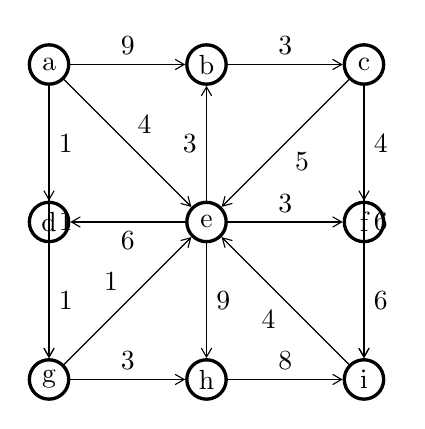
\begin{tikzpicture}[scale=2, auto]
    \tikzstyle{graph vertex} = [circle,draw=black,fill=white,very thick,inner sep=1.5pt, minimum size=5mm]
    \tikzstyle{graph edge undirected} = [draw=black]
    \tikzstyle{graph edge directed} = [graph edge undirected, ->, >=angle 60]
\node[graph vertex] (a) at (0, 2) {a};
\node[graph vertex] (b) at (1, 2) {b};
\node[graph vertex] (c) at (2, 2) {c};
\node[graph vertex] (d) at (0, 1) {d};
\node[graph vertex] (e) at (1, 1) {e};
\node[graph vertex] (f) at (2, 1) {f};
\node[graph vertex] (g) at (0, 0) {g};
\node[graph vertex] (h) at (1, 0) {h};
\node[graph vertex] (i) at (2, 0) {i};
\draw[graph edge directed] (a) to node {9} (b);
\draw[graph edge directed] (a) to node {1} (d);
\draw[graph edge directed] (a) to node {4} (e);
\draw[graph edge directed] (a) to node {1} (g);
\draw[graph edge directed] (b) to node {3} (c);
\draw[graph edge directed] (c) to node {4} (f);
\draw[graph edge directed] (c) to node {5} (e);
\draw[graph edge directed] (c) to node {6} (i);
\draw[graph edge directed] (e) to node {3} (f);
\draw[graph edge directed] (e) to node {6} (d);
\draw[graph edge directed] (e) to node {3} (b);
\draw[graph edge directed] (e) to node {9} (h);
\draw[graph edge directed] (d) to node {1} (g);
\draw[graph edge directed] (g) to node {3} (h);
\draw[graph edge directed] (g) to node {1} (e);
\draw[graph edge directed] (h) to node {8} (i);
\draw[graph edge directed] (f) to node {6} (i);
\draw[graph edge directed] (i) to node {4} (e);
\end{tikzpicture}
\end{center}
\begin{center}
\begin{tabular}{|r||c@{\,}c|c@{\,}c|c@{\,}c|c@{\,}c|c@{\,}c|c@{\,}c|c@{\,}c|c@{\,}c|c@{\,}c|}
\hline
 & & 1. & & 2. & & 3. & & 4. & & 5. & & 6. & & 7. & & 8. & & 9.\\
\hline
a & $\cdot$ & 0 & &  & &  & &  & &  & &  & &  & &  & & \\
\hline
b & $\cdot$ & $\infty$ & a & 9 & a & 9 & a & 9 & \textbf{e} & \textbf{5} & e & 5 & &  & &  & & \\
\hline
c & $\cdot$ & $\infty$ & $\cdot$ & $\infty$ & $\cdot$ & $\infty$ & $\cdot$ & $\infty$ & $\cdot$ & $\infty$ & $\cdot$ & $\infty$ & b & 8 & b & 8 & & \\
\hline
d & $\cdot$ & $\infty$ & a & 1 & &  & &  & &  & &  & &  & &  & & \\
\hline
e & $\cdot$ & $\infty$ & a & 4 & a & 4 & \textbf{g} & \textbf{2} & &  & &  & &  & &  & & \\
\hline
f & $\cdot$ & $\infty$ & $\cdot$ & $\infty$ & $\cdot$ & $\infty$ & $\cdot$ & $\infty$ & e & 5 & e & 5 & e & 5 & &  & & \\
\hline
g & $\cdot$ & $\infty$ & a & 1 & a & 1 & &  & &  & &  & &  & &  & & \\
\hline
h & $\cdot$ & $\infty$ & $\cdot$ & $\infty$ & $\cdot$ & $\infty$ & g & 4 & g & 4 & &  & &  & &  & & \\
\hline
i & $\cdot$ & $\infty$ & $\cdot$ & $\infty$ & $\cdot$ & $\infty$ & $\cdot$ & $\infty$ & $\cdot$ & $\infty$ & h & 12 & h & 12 & \textbf{f} & \textbf{11} & f & 11\\
\hline
\end{tabular}
\end{center}
\begin{center}
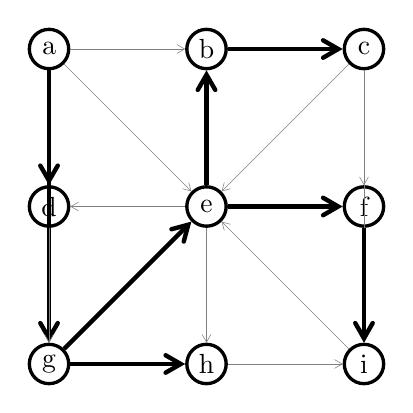
\begin{tikzpicture}[scale=2, auto]
    \tikzstyle{graph vertex} = [circle,draw=black,fill=white,very thick,inner sep=1.5pt, minimum size=5mm]
    \tikzstyle{graph edge undirected} = [draw=black]
    \tikzstyle{graph edge directed} = [graph edge undirected, ->, >=angle 60]
\node[graph vertex] (a) at (0, 2) {a};
\node[graph vertex] (b) at (1, 2) {b};
\node[graph vertex] (c) at (2, 2) {c};
\node[graph vertex] (d) at (0, 1) {d};
\node[graph vertex] (e) at (1, 1) {e};
\node[graph vertex] (f) at (2, 1) {f};
\node[graph vertex] (g) at (0, 0) {g};
\node[graph vertex] (h) at (1, 0) {h};
\node[graph vertex] (i) at (2, 0) {i};
\draw[graph edge directed, very thin, gray] (a) to (b);
\draw[graph edge directed, ultra thick] (a) to (d);
\draw[graph edge directed, very thin, gray] (a) to (e);
\draw[graph edge directed, ultra thick] (a) to (g);
\draw[graph edge directed, ultra thick] (b) to (c);
\draw[graph edge directed, very thin, gray] (c) to (f);
\draw[graph edge directed, very thin, gray] (c) to (e);
\draw[graph edge directed, very thin, gray] (c) to (i);
\draw[graph edge directed, ultra thick] (e) to (f);
\draw[graph edge directed, very thin, gray] (e) to (d);
\draw[graph edge directed, ultra thick] (e) to (b);
\draw[graph edge directed, very thin, gray] (e) to (h);
\draw[graph edge directed, very thin, gray] (d) to (g);
\draw[graph edge directed, ultra thick] (g) to (h);
\draw[graph edge directed, ultra thick] (g) to (e);
\draw[graph edge directed, very thin, gray] (h) to (i);
\draw[graph edge directed, ultra thick] (f) to (i);
\draw[graph edge directed, very thin, gray] (i) to (e);
\end{tikzpicture}
\end{center}
\end{document}
